\section{Issue \#2 and \#61: Timer for Activities}
This section concerns two issues, \#2 and \#61. Issue \#2 consists of the user story "As a citizen I want a time timer so that I know how long is left of my current activity" and issue \#61 consists of the user story "As a guardian I would like to be able to add a timer to an activity so that the citizen can see how much time is to be spent on this activity".
Full stack development played a big part in the development of these issues. Changes had to be done to both the front-end and the back-end, across three repositories: Web-api, Api-client and Weekplan \todo{Hvornår skal vi refe til vores repos?}.
Before beginning development on the user stories, we created a task list to get a better overview. The task list can be seen below:
\begin{itemize}
    \item Create Timer table in the database.
    \item Create foreign key from activity table referencing the Timer table.
    \item Change the update activity endpoint, so when an activity is updated, the timer is also updated.
    \item Reflect these changes on the api-client.
    \item Redesign the activity screen to display a timer with play-, pause- and stop-buttons for citizens and additionally a delete button for guardians. 
\end{itemize}

The following subsections each cover a part in the stack, starting with the database and web-api, then communication between server and client, and lastly the user interface.

\subsection{Implementation of Timer in Database and Updated End-point}
For the management of the models in the database and on the server, the web-api makes use of the Entity Framework. A short description of Entity Framework can be found in section~\ref{section:entityFramework}.

After discussing the design of the timer table, we came up with the following database design:

\code   {sections/4Sprint/code/sqlDatabaseMigrationTimer.txt} %Filepath
        {SQL for migration of the database.} %Caption
        {code:timerMigrationSqlDatabase} %Label
        {SQL} %Language
        
The 'Key' is database generated and auto incremented, so that all keys are unique.
'StartTime' is an integer and contains seconds since 1970-01-01, 00:00:00 UTC, called UNIX Epoch time. The reason for using unix timestamp instead of a DateTime, is that different devices, with different settings, might output conflicting DateTimes. By using unix timestamp, the start time of the timer will be universal and have no conflicting DateTimes. The 'StartTime' will be updated every time the timer goes from a paused state to a playing state. 
'Progress' is the progress based on a percentile from 0-100, saved as an integer, which will be updated every time the timer is paused.
'FullLength' is the full length of the timer in seconds. 'Paused' is a boolean value displaying whether the timer is paused or not.

Consider the example where a guardian sets a timer with a start time of 17:10:40, with a full length of 10 minutes. Since the timer has not been played yet, this results in the progress of the timer being set to 0 and the paused field being set to true, as a newly created timer starts off in a paused state.
If the timer is now started, the paused field will be changed to false. If another device loads up the same activity, the timer will be fetched from the database. As the paused field has been set to false, the new device calculates the difference from the start time in the database to that device's current time. This will be used as a local progress indicator for the device. Now the two devices will display two synchronous timers.

As mentioned in the start of the section, the web-api uses the Entity Framework. By using Entity Framework, C\# classes can be reflected in the database directly as tables, creating attributes on a table based on the fields in the class. Additionally, Entity Framework is capable of making migrations on the database that are necessary for the information to be stored. The Entity Framework abstracts from the SQL queries by using native functions in the C\# language with identical behaviour.  

It does this through two methods, one for upgrade, containing the queries for the update, and one for downgrade, which contains the queries necessary for downgrading of the database. Both methods are auto-generated, but can be manually modified to reach expected behaviour.
In order to reflect the changes shown in code~snippet~\ref{code:timerMigrationSqlDatabase}, the classes in the web-api need to be modified. The timer class needs to be created in order to represent the timer table in the database. Furthermore, the activity class needs to be modified to contain a timer key referencing the key of a timer in the timer table. The timer class can be seen in code~snippet~\ref{code:timerWebApi}.

\code   {sections/4Sprint/code/timerDatabase.txt} %Filepath
        {The timer defined in the web-api.} %Caption
        {code:timerWebApi} %Label
        {C} %Language

After the migration of the database, the endpoints related to the activity containing a timer should be updated  in the web-api accordingly. These changes should be done to the 'UpdateActivity'- and the 'ReadUsersWeekSchedule'-endpoint.

In the 'UpdateActivity'-endpoint the following additions have been made:
\code   {sections/4Sprint/code/updateActivityEndpoint.txt} %Filepath
        {Updates done to the 'UpdateActivity'-endpoint. The full method can be found in appendix~\ref{code:updateActivityFull}.} %Caption
        {code:UpdateActivityEndPoint} %Label
        {C} %Language
        
The endpoint on the web-api receives the activity from the body of the HTTP request, represented as json. In the body the method for updating an activity, we inserted the code seen on code~snippet~\ref{code:UpdateActivityEndPoint}. The 'activity' variable is the one received from the body. The 'updateActivity' variable is the entry in the database that needs to be updated. Firstly, if a timer already exists on the current activity, the timer is fetched from the database and its values are updated. If not, a new timer object is created on the activity, and its values are updated.
However, if the activity is updated without any timer, the 'TimerKey' of 'UpdateActivity' will be removed and the timer is deleted from the database.

In the 'ReadUsersWeekSchedule'-endpoint the following additions have been made:
\code   {sections/4Sprint/code/weekEndpointUpdate.txt} %Filepath
        {Updates done to the 'ReadUsersWeekSchedule'-endpoint. The full method can be found in appendix~\ref{code:readUsersWeekScheduleFull}.} %Caption
        {code:ReadUsersWeekScheduleEndPoint} %Label
        {C} %Language

'ReadUsersWeekSchedule' is used to get one week belonging to a user, with its days containing the activities. In this method, the code from code~snippet~\ref{code:readUsersWeekScheduleFull} was added.
Instead of just returning the week as it is, the week's activities are individually updated with a related timer if one exists. From this, the timer can be found in the activity object when 'UpdateActivity' is called.

The full methods can be found in respectively appendix~\ref{code:updateActivityFull} and appendix~\ref{code:readUsersWeekScheduleFull}.

\subsection{Update Communication Between Server and Client}
The api-client is responsible for representing the model to the front-end of the applications. Therefore a timer class was added to the api-client and the activity class was updated with the timer. The timer class contains a toJson and a fromJson method. The toJson method is used to convert an object into json for when an activity is requested from the server, and the fromJson is used to convert json from the response from the server back into an object. The full representation of the timer class can be seen in code~snippet in appendix~\ref{code:timerClassFlutter}.

\subsection{Update User Interface with Timer}
The design of the timer followed the prototypes, additional requirements were found through a conversation with the PO-group. The timer was requested to be integrated in the activity screen, so the timer for an activity is shown when the activity is tapped on in the weekplan screen. As mentioned earlier, two issues were involved, one regarding a timer in guardian mode and the other in citizen mode. This meant that the design of the user interface should depend on the mode that the application is in. 

First, it should be possible to add a timer to an activity, but only when in guardian mode. Therefore we had to only show the "Add timer"-button, when the device was in guardian mode, and show nothing when the device was in citizen mode, as seen on figure~\ref{fig:addTimerGuardian} and figure~\ref{fig:addTimerCitizen} respectively. 

\begin{figure}[H]
\minipage{0.48\textwidth}
  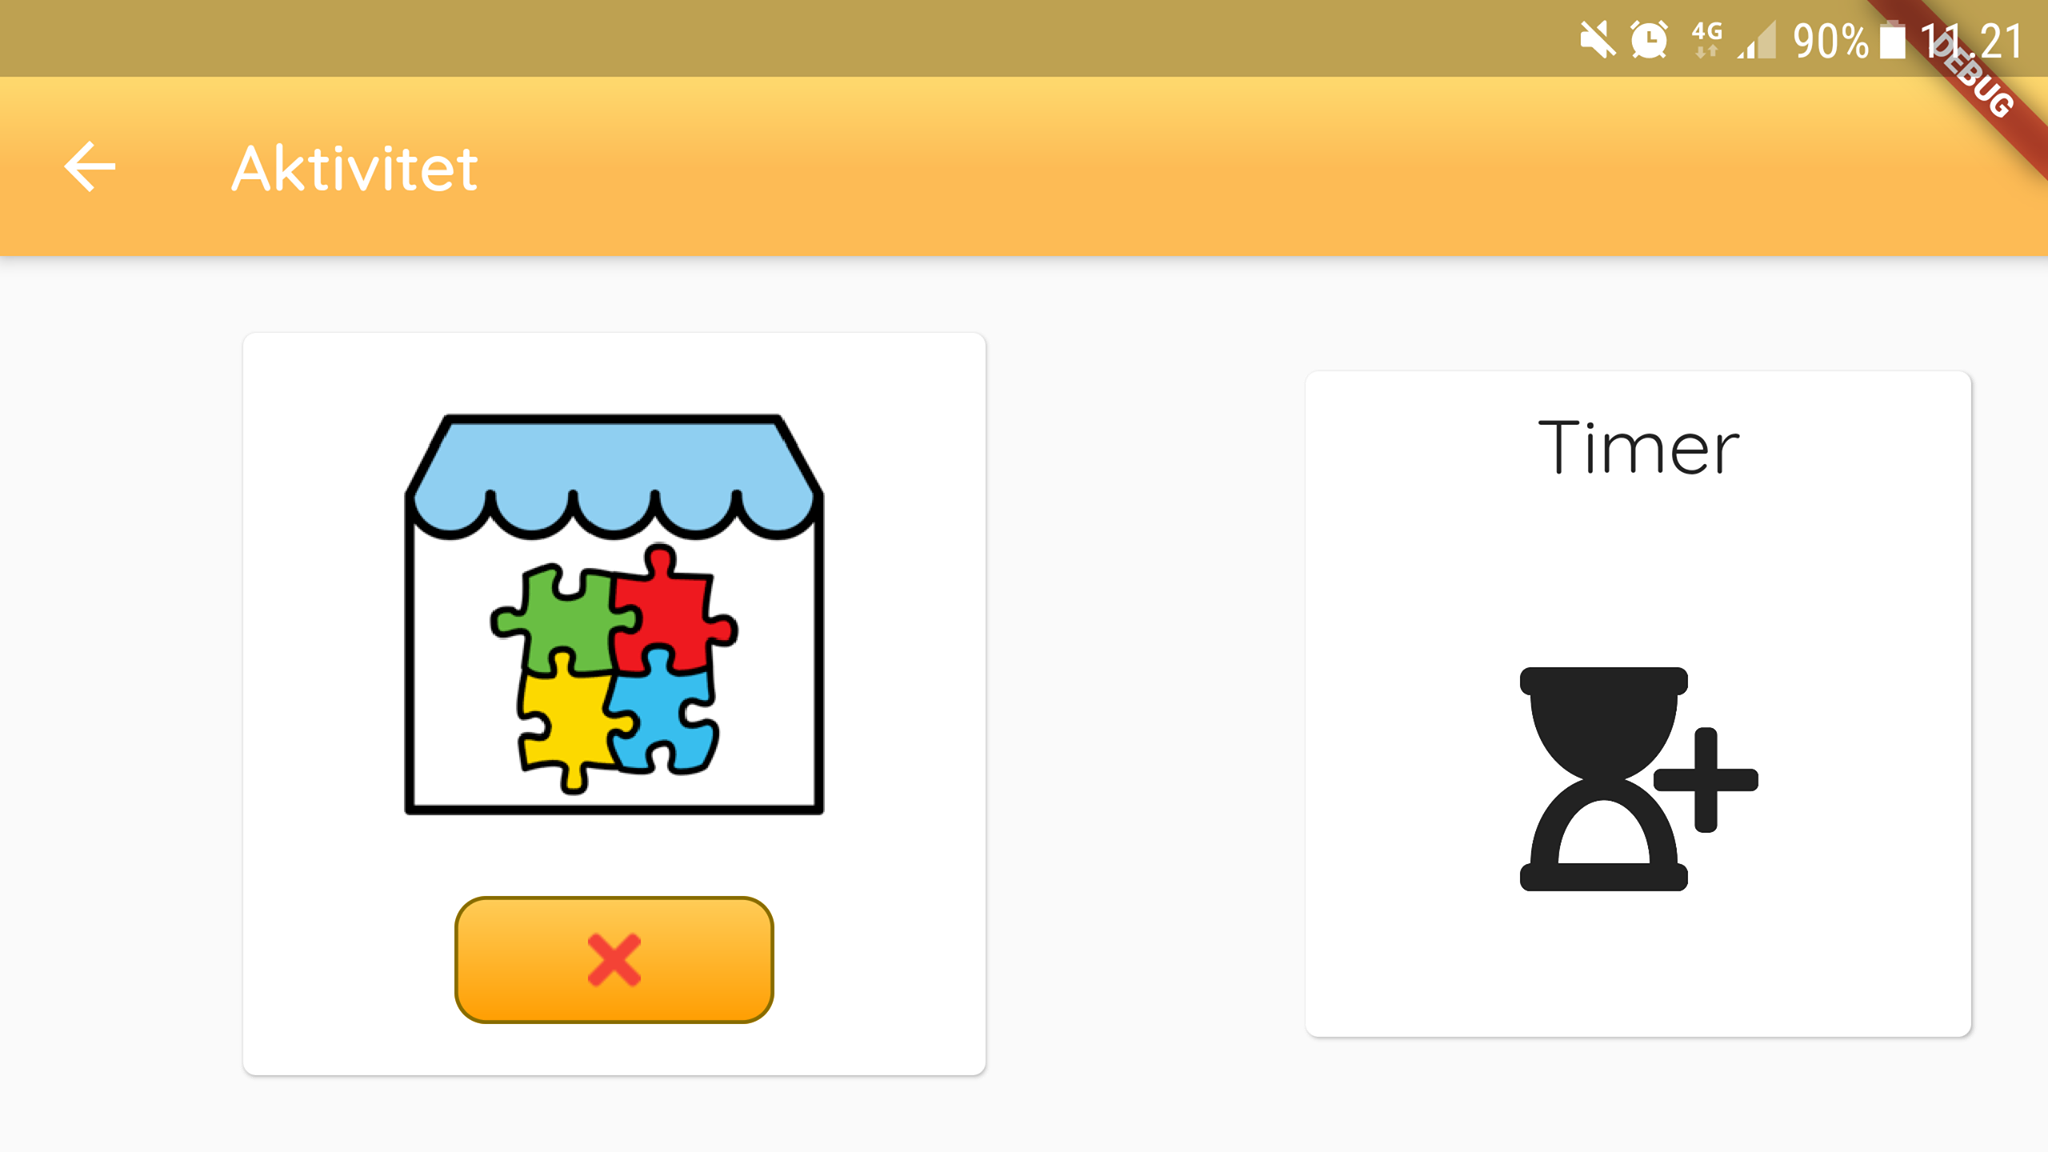
\includegraphics[width=\linewidth]{sections/4Sprint/images/addTimerGuardian.png}
  \caption{Activity screen guardian mode.}
  \label{fig:addTimerGuardian}
\endminipage\hfill \quad
\minipage{0.48\textwidth}
  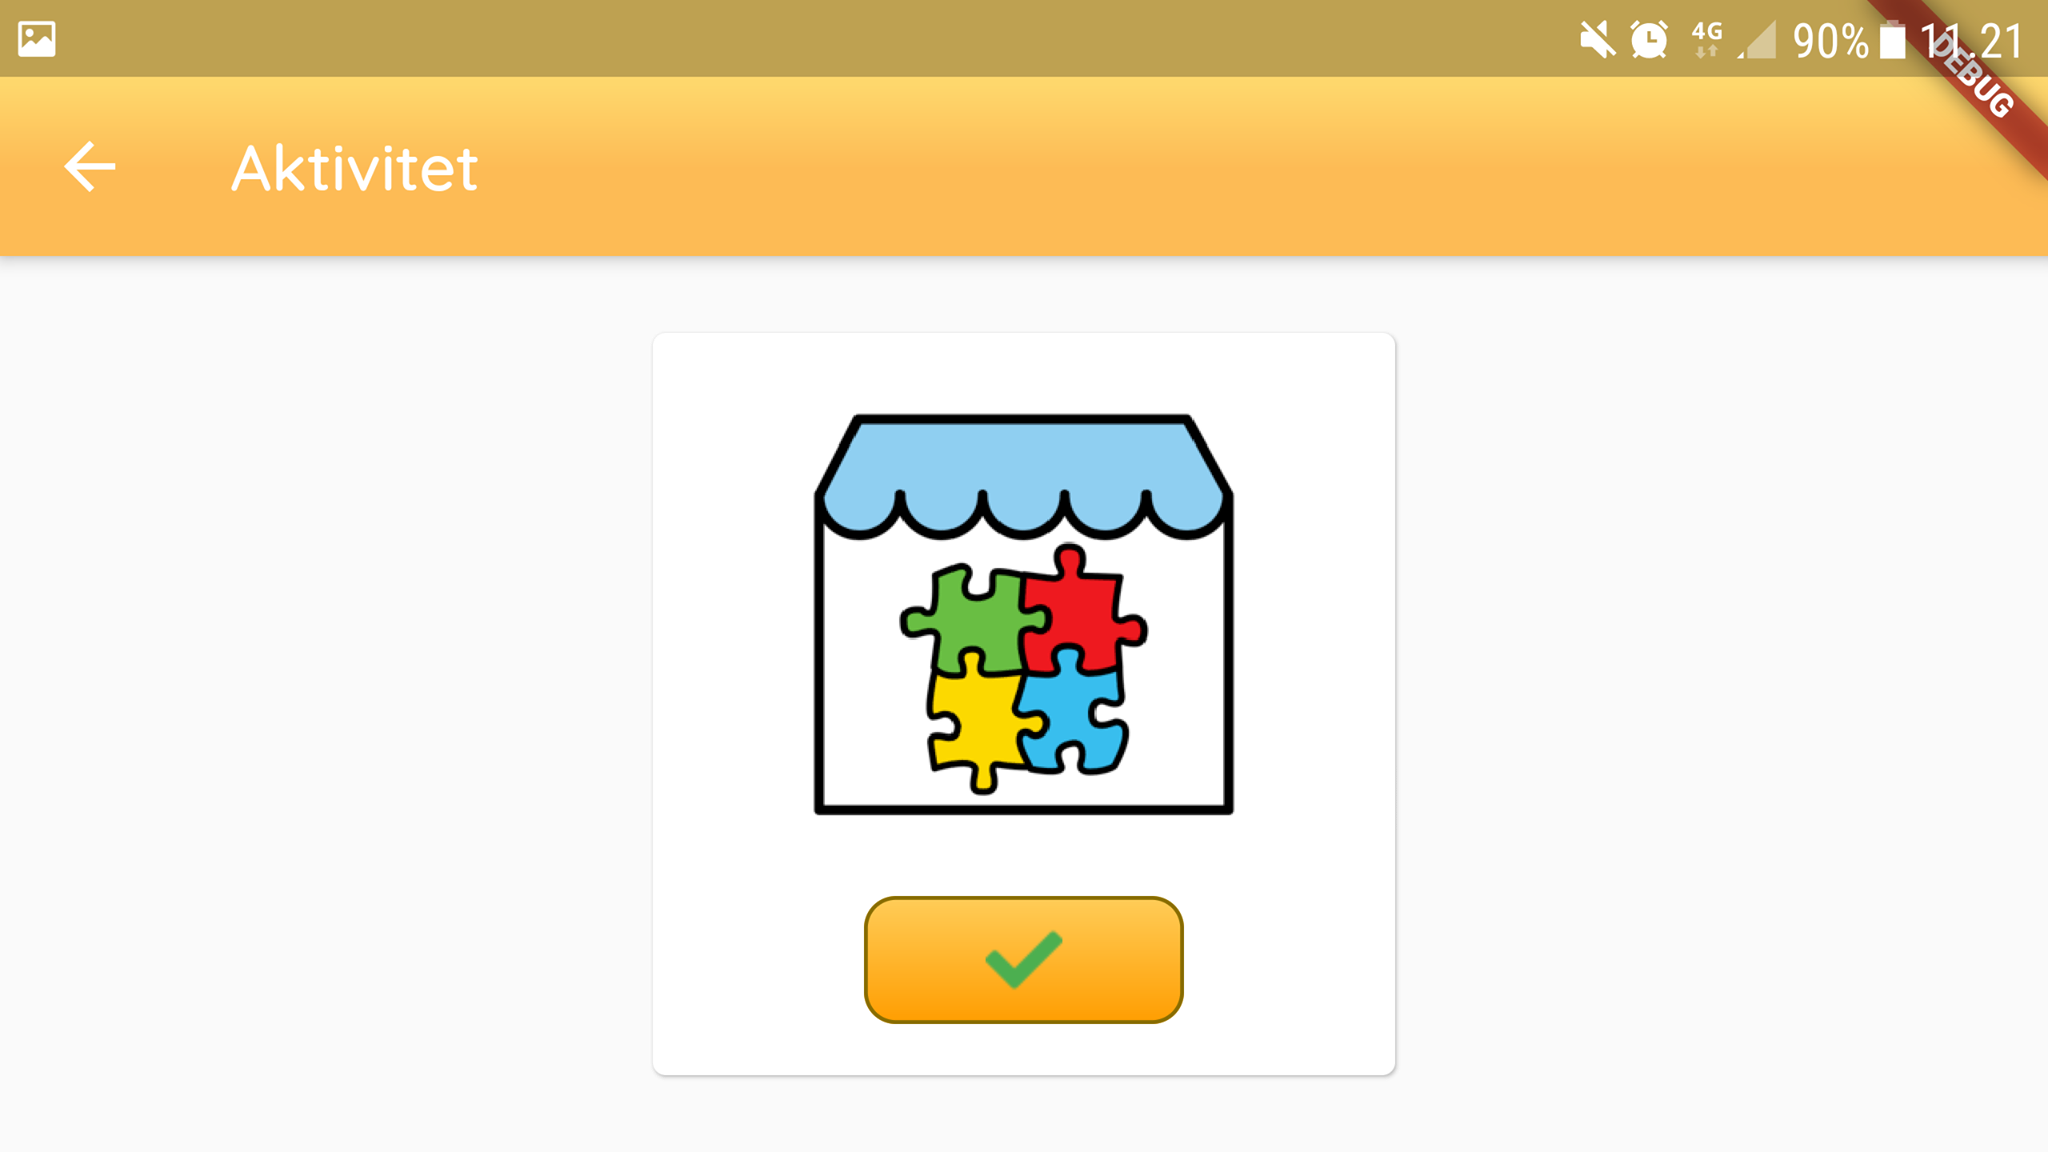
\includegraphics[width=\linewidth]{sections/4Sprint/images/addTimerCitizen.png}
  \caption{Activity screen citizen mode.}
  \label{fig:addTimerCitizen}
\endminipage\hfill
\end{figure}

As mentioned, when in guardian mode, it was possible to add a timer to the activity. When pressing the add timer button, the user was prompted with a dialog, requiring the user to enter the duration the timer should run for. The dialog for choosing the time can be seen on figure~\ref{fig:timePickerDialog}, with text fields for hours, minutes and seconds. To begin with, the plan was to have various timer indications to choose from, as seen on the prototype on figure~\ref{fig:timePickerPrototype}. However, the PO-group decided that we should only implement the circular timer, so the choice of time indication was excluded in our dialog.

\begin{figure}[H]
\center
\minipage{0.37\textwidth}
  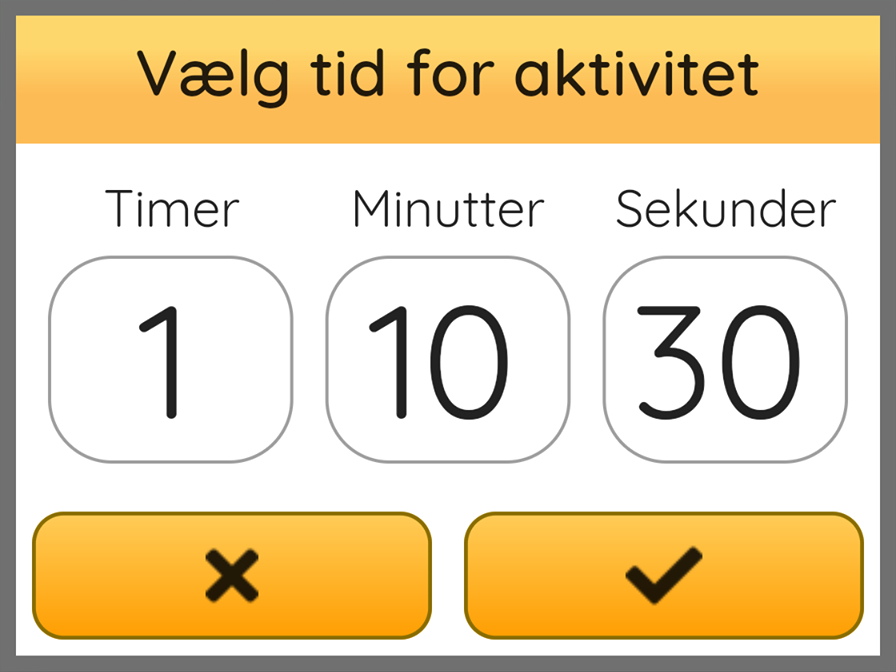
\includegraphics[width=\linewidth]{sections/4Sprint/images/timePicker.png}
  \caption{Time Picker Dialog.}
  \label{fig:timePickerDialog}
\endminipage\hfill \quad
\minipage{0.56\textwidth}
  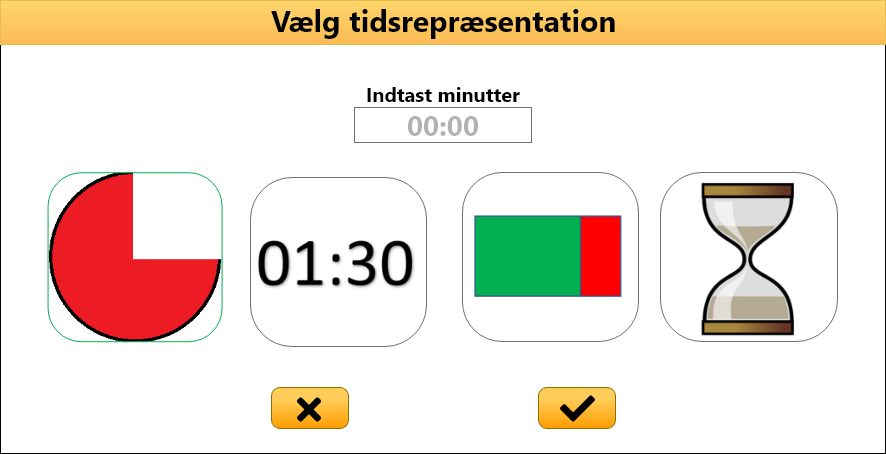
\includegraphics[width=\linewidth]{sections/4Sprint/images/prototypeTimerPicker.png}
  \caption{Time Picker Dialog Prototype.}
  \label{fig:timePickerPrototype}
\endminipage\hfill
\end{figure}

If the user has entered a valid time in the fields, a timer is created for the activity. 
The actions available for the timer varies whether the device is in guardian or citizen mode. 
The screens with a created timer for guardian mode and citizen mode can be seen on figure~\ref{fig:timerButtonsGuardian} and figure~\ref{fig:timerButtonsCitizen} respectively.

\begin{figure}[H]
\center
\minipage{0.40\textwidth}
  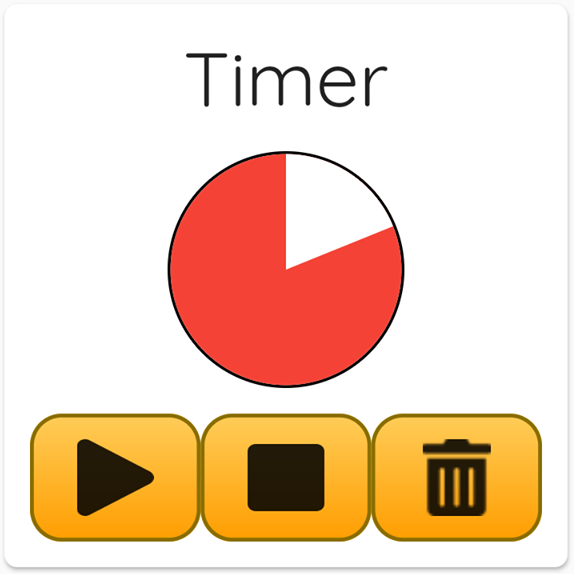
\includegraphics[width=\linewidth]{sections/4Sprint/images/timerButtonsGuardian.png}
  \caption{Buttons shown i guardian mode.}
  \label{fig:timerButtonsGuardian}
\endminipage \quad
\minipage{0.40\textwidth}
  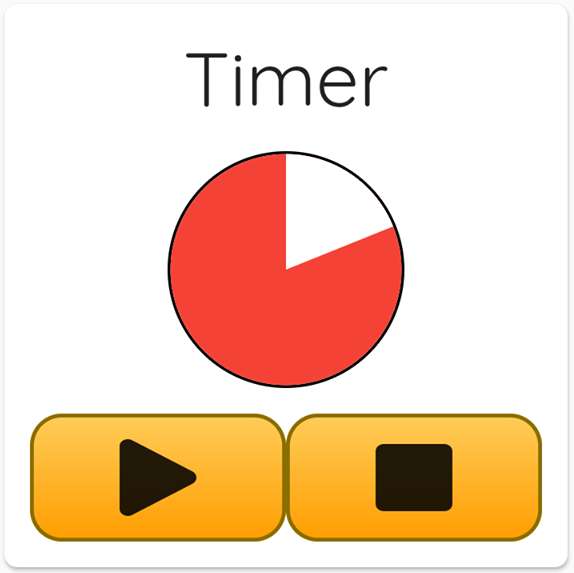
\includegraphics[width=\linewidth]{sections/4Sprint/images/timerButtonsCitizen.png}
  \caption{Buttons shown i citizen mode.}
  \label{fig:timerButtonsCitizen}
\endminipage
\end{figure}

When in guardian mode, the user has the options to play/pause, stop and delete the timer. When the device is in citizen mode, the user only has the options to play/pause and stop the timer. The stop and delete actions prompt the user with a confirmation dialog, asking if they are certain they want to continue. This is to prevent the user from mistakenly clicking a wrong button and losing the progress of the timer.